\section{Evaluation}
In this section, we use a set of experiments to show that
given an interested SDN (sub)network with rules $SN(R)$, our approach can 
(1) transform $SN(R)$ to a single OpenFlow switch without any loss of forwarding logic in network $SN(R)$;
(2) save emulation resources such as number of total rules in the network and emulation runtime.

We consider a tree-topology network with two topological parameters: depth $d$ and fanout $f$.
Such a tree network $tree(d, f)$ can connect $f^d$ hosts with $\frac{f^d - 1}{f-1}$ switches in total.
Though not known as a scalable network architecture
(a good scalable alternative will be fat-tree topology),
it is good for demonstration purpose since the tree topology is well-structured and
all hosts in it are potentially fully-connected with at most $2d$ hops.

\subsection{Preserve Forwarding Rule Equivalence}
\label{SubSec:PreserveForwardingLogic}

\begin{figure*}[t]
        \centering
        \subfloat[Packets received in $net_1(d=2, f=3)$] {
                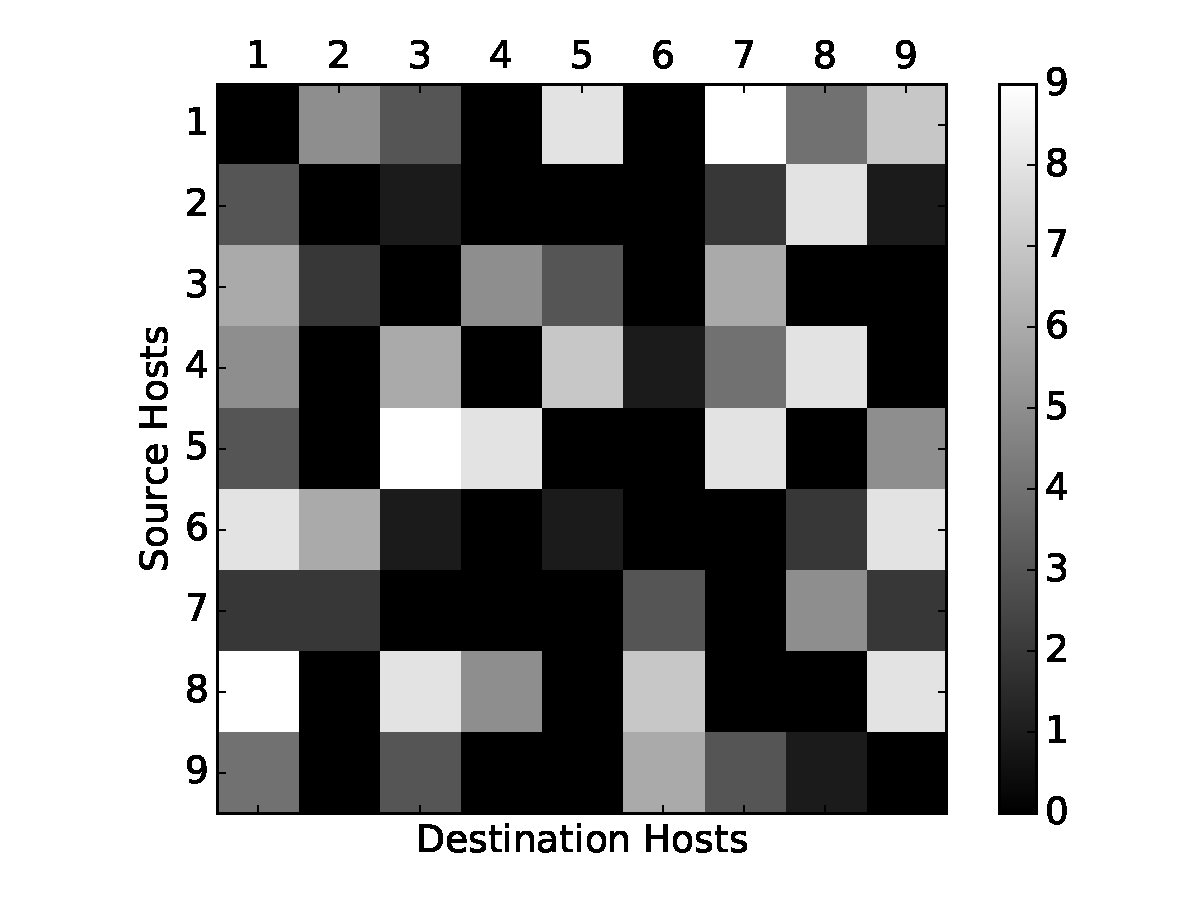
\includegraphics[scale=.42]{figures/ping_mat_2_3.pdf}
                \label{Fig:PingMatrix1}
        }
        \subfloat[Packets received in $net_2(d=2, f=3)$] {
                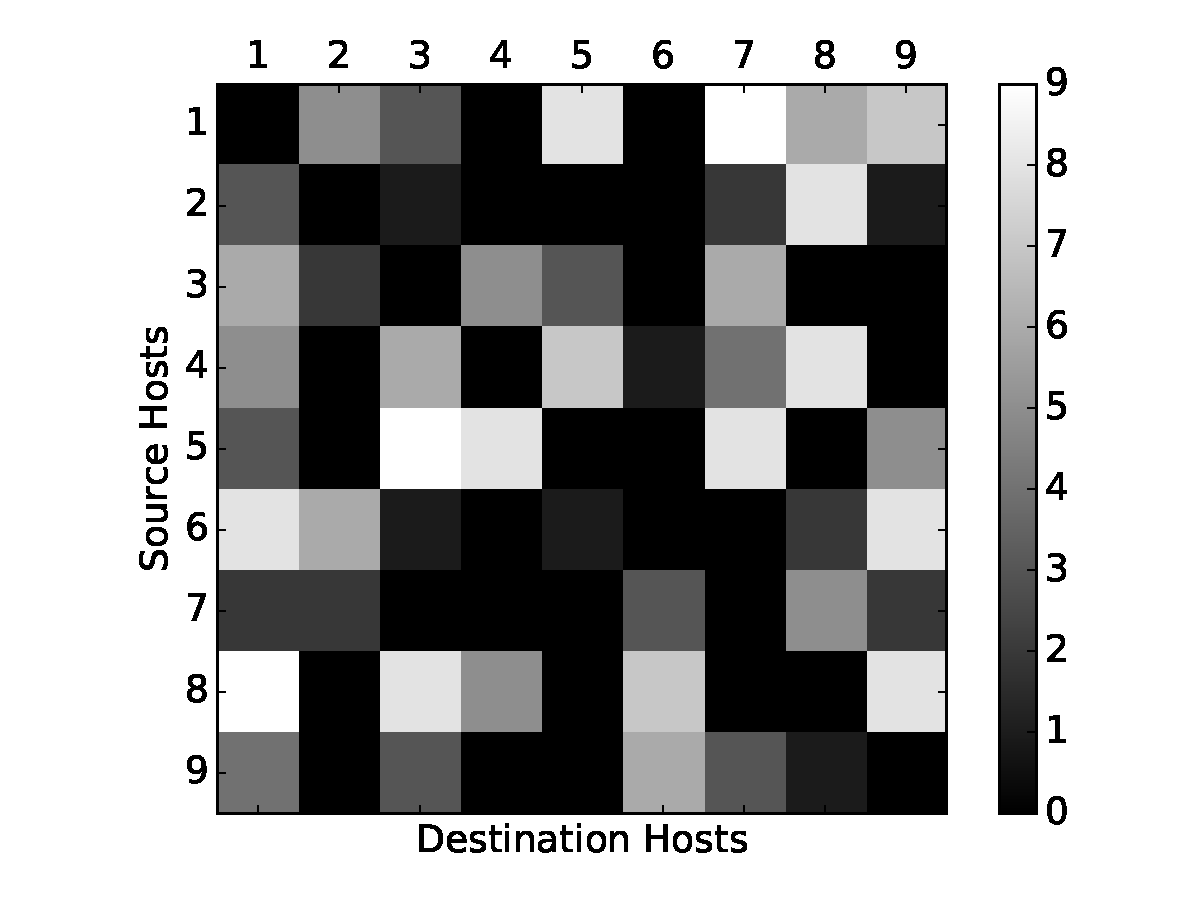
\includegraphics[scale=.42]{figures/bs_ping_mat_2_3.pdf}
                \label{Fig:PingMatrix2}
        }
        \\
        \subfloat[Packets received in $net_1(d=4, f=3)$] {
                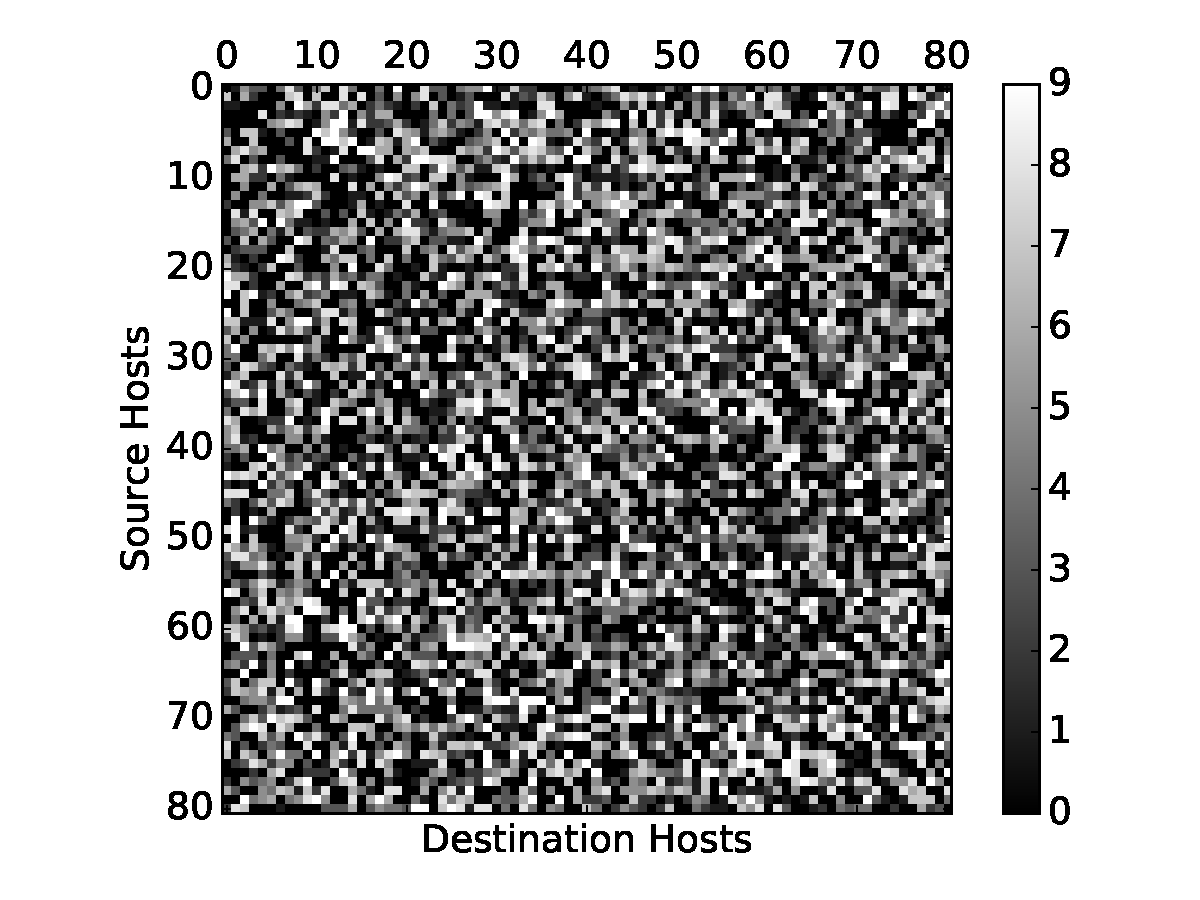
\includegraphics[scale=.42]{figures/ping_mat_4_3.pdf}
                \label{Fig:PingMatrix3}
        }
        \subfloat[Packets received in $net_2(d=4, f=3)$] {
                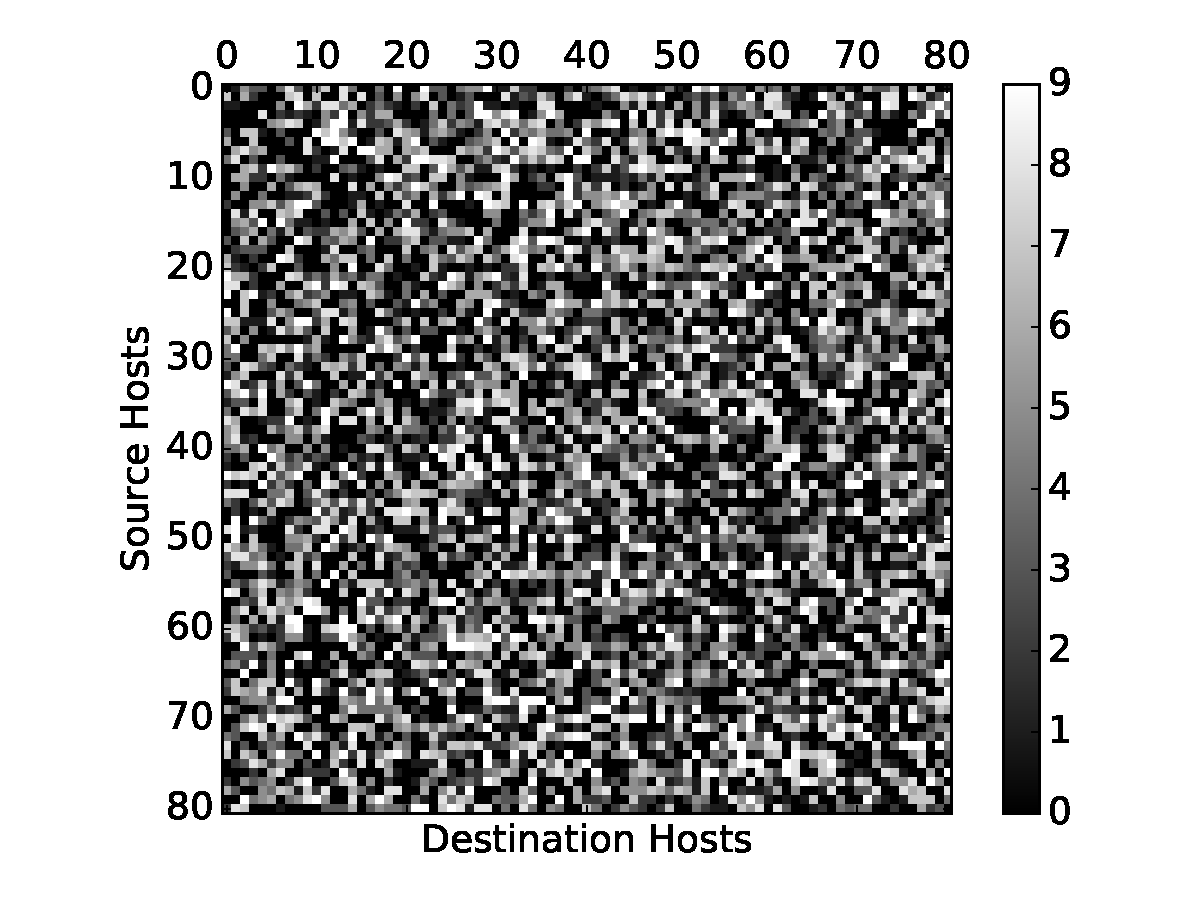
\includegraphics[scale=.42]{figures/bs_ping_mat_4_3.pdf}
                \label{Fig:PingMatrix4}
        }
        \caption{Comparing $\mathcal{R}_1$ and $\mathcal{R}_2$ of two emulated networks as
        gray image}
        \label{Fig:ComparePingMatrix}
\end{figure*}

In the following set of experiment, we demonstrate that forwarding logic in $SN(R)$ are
perfectly preserved by the big-virtual-switch approach.
We generate forwarding logic in tree-topology network by create paths between random host pairs.
One can find the shortest path between a pair of hosts $(s, d)$ with
a layer-two learning switch controller application.
Traversing the tree up and down in breadth-first-search style, learning switch application
can automatically install OpenFlow rules on each hop once we initiate \texttt{ping} between
the given pair of host.
More specifically, we start a tree-topology network $net_1$ in Mininet\cite{Mininet},
connecting all switches to a l2\_learning switch controller\cite{Pox}.
For any network host $s$, we randomly generate a list of distinct hosts $dsts$,
and let $s$ \texttt{ping} each host $dst \in dsts$.
After doing this \texttt{ping} process for all hosts, necessary rules will be available on
certain switches.
We then take a snapshot of this network by
\begin{enumerate}
\item Recording the network topology, e.g. host to switch and switch to switch connections.
\item Logging all rules on all switches with \texttt{ovs-ofctl dump-flows} commands
\end{enumerate}
We then feed the above information as input in order to generate the rules of the new big switch
and port mappings according to procedures and algorithms presented in section~\ref{Sec:Design}.
Now we create another emulated network with one switches and
the same number of hosts as $net_1$ using Mininet.
This big-switch network $net_2$ has one OpenFlow switch $bs$ that connects to $f^d$ hosts using
appropriate port numbers deducted from both the $PortMap$(from Algorithm~\ref{Alg:GenAllRules})
and link information(from $net_1$'s topology record).
Besides, rules generated by Algorithm~\ref{Alg:GenAllRules} are manually(instead by controller)
installed on $bs$ by \texttt{ovs-ofctl add-flow} commands.

To proof that our approach can preserve the existing forwarding logic in original network,
we generate a matrix $\mathcal{M}$ of size $f^d$ by $f^d$, each element randomly picked
from the integer range [1, 10].
In both emulated network $net_1$ and $net_2$, host $i$ will send $\mathcal{M}[i][j]$
packets to host $j$ using \texttt{ping}, if $i \neq j$.
To prevent l2\_learning switch controller from installing new rules in $net_1$, we take down
the pox controller in this stage.
The result of this experiment is a matrix $\mathcal{R}_k$ where $\mathcal{R}[i][j]$ denote
the number of successfully received \texttt{ping} packets by host $i$ from host $j$ in $net_k$.

We have repeated this experiment for different ($d, f$) pairs $\in$
\{(2, 3), (2, 4), (3, 3), (3, 4), (4, 3)\} and, for each experiment setting,
we save the experiment result $\mathcal{R}_1$ and $\mathcal{R}_2$
as text in order to compare them using \texttt{diff} command.
We found that $\mathcal{R}_1 = \mathcal{R}_2$ holds in all five experiment settings.
As an example, we visualize $\mathcal{R}_1$ and $\mathcal{R}_2$ for both ($d=2, f=3$)
and ($d=4, f=3$) as gray image in Figure~\ref{Fig:ComparePingMatrix}.
In Figure~\ref{Fig:PingMatrix1}-Figure~\ref{Fig:PingMatrix4},
the pixels' brightness is proportional to $\mathcal{R}[i][j]$,
the number of returned packets sending out from host $i$ and echoed back from host $j$.
In this way it is easy to see that $\mathcal{R}_1$ and $\mathcal{R}_2$ are identical
indeed for all experiment settings.

\subsection{Speedup Simulation}

\begin{figure}[h]
\centering
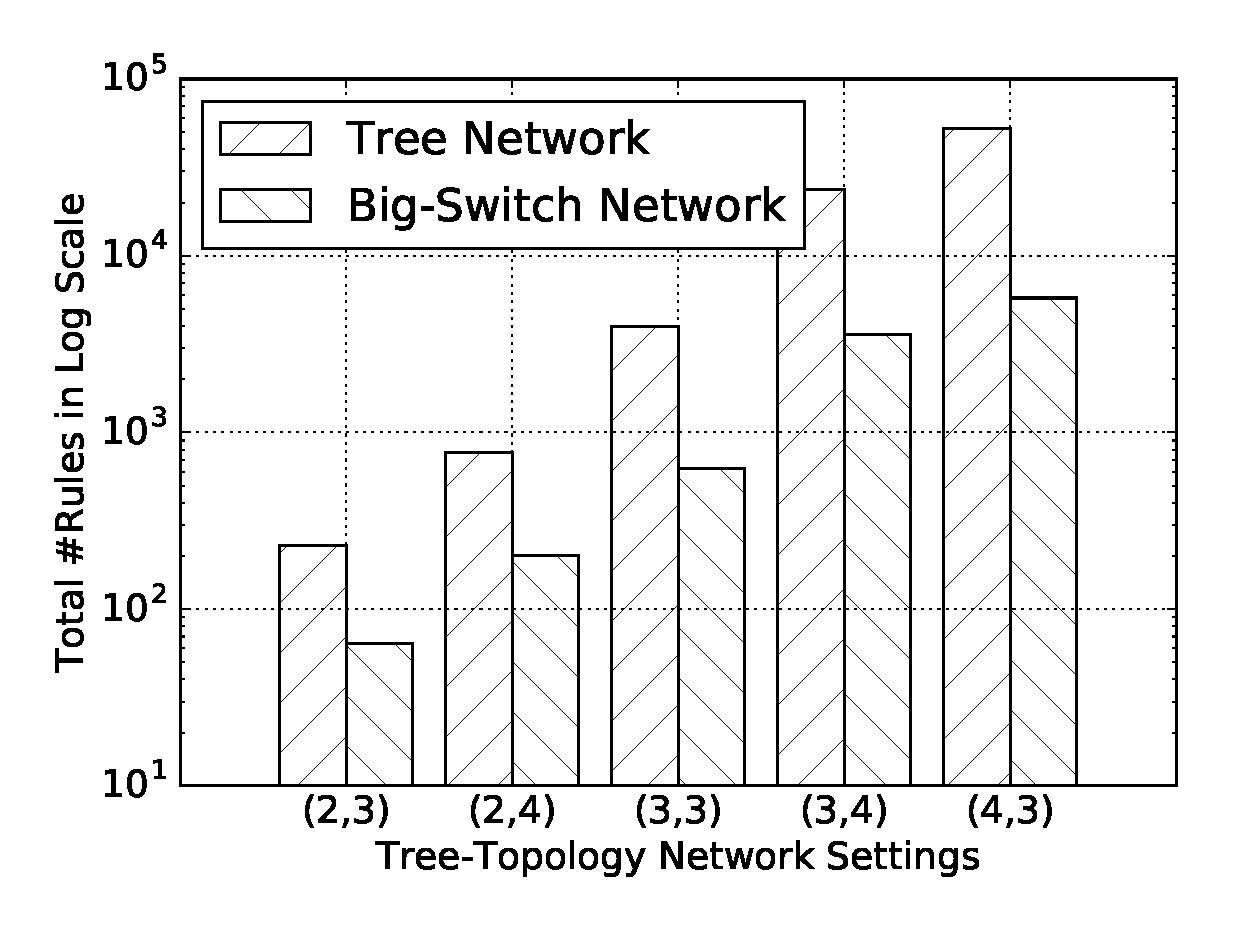
\includegraphics[scale=.42]{figures/comp_num_rules.eps}
\caption{The number of rules on big switch is approximately \textbf{one tenth} of the
        number of rules existing in the tree-topology network.
        The label on x-axis represents the tree-topology's depth and fanout parameters.}
\label{Fig:CompareNumRules}
\end{figure}

\begin{figure}[h]
\centering
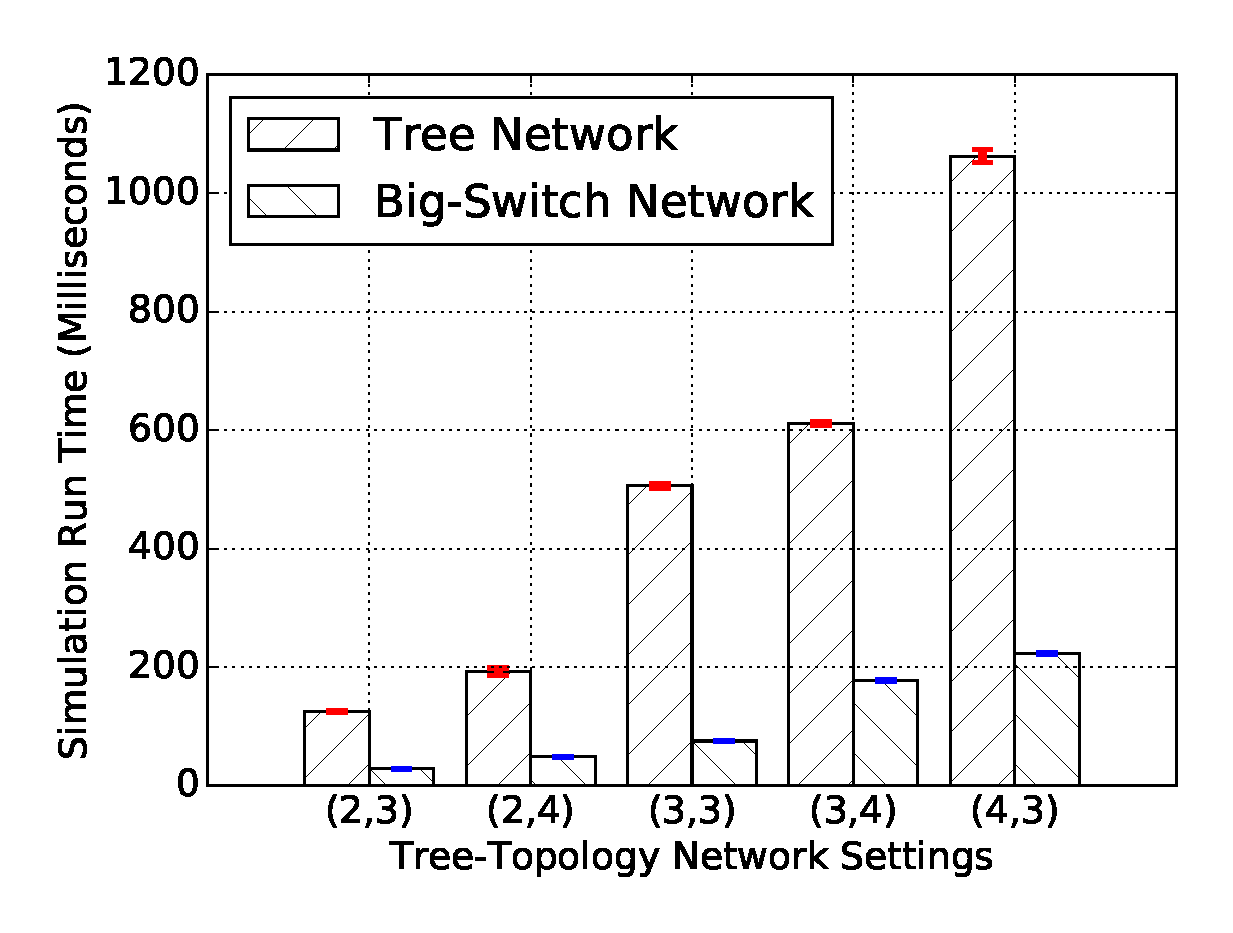
\includegraphics[scale=.42]{figures/comp_sim_time.eps}
\caption{Using our Big-Switch network model, S3FNet can save about 80\% run time
        comparing to simulating the tree-topology network.
        The label on x-axis represents the tree-topology's depth and fanout parameters.}
\label{Fig:CompareSimulationTime}
\end{figure}

During the running of this group of experiments,
we collected the total number of rules in the snapshot of the network in both $net_1$
and $net_2$.
The results are plotted in Figure~\ref{Fig:CompareNumRules} for different
topological parameter settings respectively.
Notice that y-axis is in log scale.
The number of rules on big switch is approximately one degree of magnitude less
than the number of rules existing in the original tree-topology network.
For example, in the case of (4, 3) 53260 rules are reduced to 5766 rules.
The benefit of our approach is that both number of switches and number of rules needed
for simulation/emulation are significantly reduced.
This will have implications on the running time of the simulation/emulation.
To show that simplied model and reduced rules can save simulation time, we conduct
the same set of experiments on network simulator S3FNet\cite{S3F}.
That is, we build two SDN networks, one for tree-topology network $net_1(d, f)$
one for the big-switch network $net_2$, separately in S3FNet.
During the simulations, we set half of the hosts as TCP clients
and the other half as TCP servers such that client $i$ requests TCP traffic from server $i$.
All the communications last 100 real-clock seconds.
We record the simulation run time for both $net_1$ and $net_2$ for different experiment
settings and compare the average results of ten runs of each settings
in Figure~\ref{Fig:CompareSimulationTime}.
The error bar shows the standard deviation of ten independent simulation runs.
In average, running big-switch network speedups 4.63 times as
running the tree-topology network.


\subsection{Overhead of Our Approach}

\begin{figure}[t]
\centering
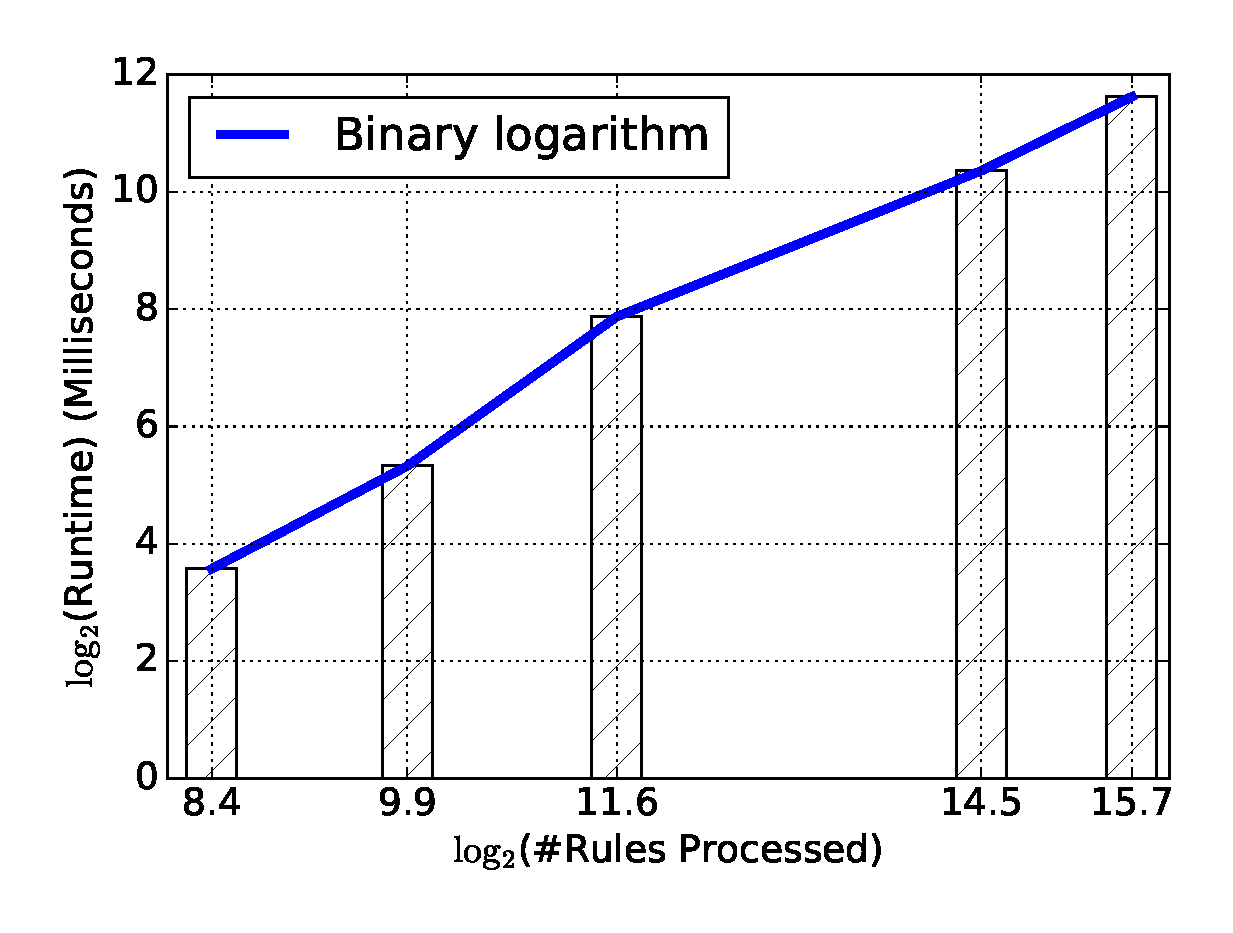
\includegraphics[scale=.42]{figures/bs_overhead.eps}
\caption{The running time overhead of our approach scales linear with the number of
        rules it needs to process.}
\label{Fig:BSOverhead}
\end{figure}

The overhead of our approach is that we need to process the existing rules in original network,
map the original topology to a single-switch topology, and
generate new rules.
In practice this process can be done offline once, as we did in the experiments above,
and the newly generated rule can be installed in multiple runs thereafter.
We have discussed our approach's asymptotic time complexity at several places in Section~\ref{Sec:Design}.
Here we show the running time $rt$ of the three-step approach with regard to
the number of rules it processed $nr$ in the logic-preserving experiment.
Since the scale of the experiment increases exponentially, we put both x-axis($nr$)
and y-axis ($rt$) in binary log scale ($\log_2$).
For the largest input size $nr=53260$, abstracting a tree network with depth 4 and
fanout 3 finishes in 3.15 seconds.
In Figure~\ref{Fig:BSOverhead}, it is clear that our approach scale linearly as the
input size increases in the scenario of this tree-topology network.
The overall processing overhead experienced in this experiment is tolerable for online use.

